\documentclass[12pt]{article}
\usepackage[left=0.25cm,top=1cm,right=0.25cm,bottom=1cm]{geometry}
\textwidth = 20cm
\hoffset = -1cm
\usepackage[utf8]{inputenc}
\usepackage[spanish,es-tabla]{babel}
\usepackage[autostyle,spanish=mexican]{csquotes}
\usepackage[tbtags]{amsmath}
\usepackage{nccmath}
\usepackage{amsthm}
\usepackage{amssymb}
\usepackage{graphicx}
\usepackage{standalone}
\usepackage[outdir=./]{epstopdf}
\usepackage{siunitx}
\usepackage{physics}
\usepackage{color}
\usepackage{float}
\usepackage{multicol}
%\usepackage{milista}
\usepackage{enumitem}
\usepackage{anyfontsize}
\usepackage{anysize}
\usepackage{enumitem}
\usepackage{capt-of}
\usepackage{bm}
\usepackage{relsize}
\usepackage{placeins}
\usepackage{empheq}
\usepackage{cancel}
\usepackage{wrapfig}
\spanishdecimal{.}
\renewcommand{\baselinestretch}{1.5} 
\renewcommand\labelenumii{\theenumi.{\arabic{enumii}}}
\newcommand{\ptilde}[1]{\ensuremath{{#1}^{\prime}}}
\newcommand{\stilde}[1]{\ensuremath{{#1}^{\prime \prime}}}
\newcommand{\ttilde}[1]{\ensuremath{{#1}^{\prime \prime \prime}}}
\newcommand{\ntilde}[2]{\ensuremath{{#1}^{(#2)}}}


\title{Enunciados del Tema 4 para el Segundo Examen \\[0.3em]  \large{Matemáticas Avanzadas de la Física}\vspace{-3ex}}
\author{M. en C. Gustavo Contreras Mayén}
\date{ }
\begin{document}
\vspace{-4cm}
\maketitle
\fontsize{14}{14}\selectfont

\textbf{Indicaciones: } Deberás de resolver cada ejercicio de la manera más completa, ordenada y clara posible, anotando cada paso así como las operaciones involucradas. El puntaje de cada ejercicio es de \textbf{1 punto}, con excepción en donde se indica.
\par
En esta ocasión se presentan siete enunciados, se seleccionarán oportunamente los seis enunciados para el Segundo Examen.

\begin{enumerate}
\item De la lectura del artículo de Michael Berry: ¿cuál es tu opinión sobre lo especial de las funciones especiales?
%Ref. Arfken (2006) 12.1.3
\item Demuestra que el potencial electrostático producido por una carga $q$ en $z = a$ para $r < a$ es:
\begin{align*}
\varphi(\vb{r}) = \dfrac{q}{4 \pi \epsilon_{0} a} \, \nsum_{n=0}^{\infty} \left( \dfrac{r}{a} \right)^{n} \, P_{n}(\cos \theta)
\end{align*}
\item Una esfera conductora de calor de radio $a$ está compuesta por dos hemisferios con un espacio infinitesimal aislante entre ellos, como se muestra en la figura (\ref{fig:figura2}). Las mitades superior e inferior de la esfera están en contacto con baños térmicos de temperaturas $+ T_{1}$ y $-T_{1}$, respectivamente. La esfera de radio $a$ está dentro de otra esfera conductora de calor de radio $b$ con una temperatura $T_{2}$.
\begin{figure}[H]
    \centering
   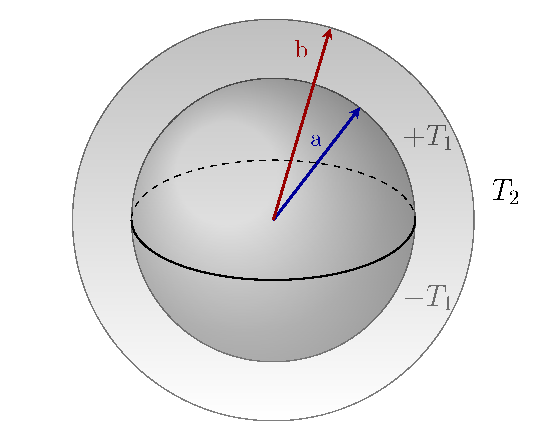
\includegraphics[scale=0.9]{Imagenes/esfera1.eps}
    \caption{Los hemisferios de la esfera interior se encuentran a diferentes temperatura.}
    \label{fig:figura2}
\end{figure}
Calcula la temperatura:
\begin{enumerate}[label=\roman*)]
\item Dentro de la esfera interior,
\item En la región entre las dos esferas, y
\item Por fuera de la esfera exterior.
\end{enumerate}
%Ref. Arfken (2006) 12.7.5
\item Verifica mediante cálculo explícito que:
\begin{align*}
L_{-} \, Y_{1}^{0} (\theta, \varphi) = + \sqrt{\dfrac{3}{4 \pi}} \, \sin \theta \, e^{-i \varphi} = \sqrt{2} \, Y_{1}^{-1} (\theta, \varphi)
\end{align*}
Estos signos (fase de Condon-Shortley) son una consecuencia de los operadores sucesivos $L_{+}$ y $L_{-}$.
%Ref.
\item Demuestra que:
\begin{align*}
P_{2n}^{1} (0) &= 0 \\[0.5em]
P_{2n+1}^{1} (0) &= (-1)^{n} \, \dfrac{(2 \, n +1)!}{(2^{n} \, n!)^{2}} = (-1)^{n} \, \dfrac{(2 \, n + 1)!!}{(2 \, n)!!}
\end{align*}
ocupando \textbf{ocupando cada uno} de los siguientes tres métodos:
\begin{enumerate}[label=(\alph*)]
\item Usando relaciones de recurrencia.
\item Expandiendo la función generatriz.
\item Mediante la fórmula de Rodrigues.
\end{enumerate}
%Ref. Arfken (2006) 12.2.11
\item La amplitud de una onda dispersada está dada por
\begin{align*}
f(\theta) = \dfrac{1}{k} \, \sum_{\ell = 0}^{\infty} (2 \, \ell + 1) \, \exp(i \, \delta_{\ell}) \, \sin \delta_{\ell} \, P_{\ell} (\cos \theta)
\end{align*}
Donde $\theta$ es el ángulo de dispersión, $\ell$ es el valor propio del momento angular, $\hbar \, k$ es el momento incidente, y $\delta_{\ell}$ es el desplazamiento de fase producido por el potencial central que está haciendo la dispersión. La sección transversal total es:
\begin{align*}
\sigma_{\text{tot}} = \int \abs{f(\theta)}^{2} \dd{\Omega}
\end{align*}
Demuestra que
\begin{align*}
\sigma_{\text{tot}} = \dfrac{4 \, \pi}{k^{2}} \sum_{\ell=0}^{\infty} (2 \, \ell + 1) \, \sin^{2} \delta_{\ell}
\end{align*}
%Ref. Arfken (2006) 12.4.2
% \item Usando la fórmula de Rodrigues, de muestra que los $P_{n} (x)$ son ortogonales y que:
% \begin{align*}
% \scaleint{6ex}_{\bs -1}^{1} \big[ P_{n} (x) \big]^{2} \dd{x} = \dfrac{2}{2 n + 1}
% \end{align*}
% Tip: Ocupa la fórmula de Rodrigues e integra por partes.
%Ref. Hassani (2009) Problem 26.26
\item Una esfera conductora de calor de radio $a$ está compuesta de dos hemisferios y una banda infinitesimal aislante entre ellos. Los hemisferios superior e inferior de la esfera están en contacto con baños térmicos de temperaturas $+T_{1}$ y $-T_{1}$, respectivamente. Dentro de la esfera de radio $a$, hay una segunda esfera conductora de radio $b$ que se mantiene a una temperatura $T_{2}$.
\begin{figure}[H]
    \centering
   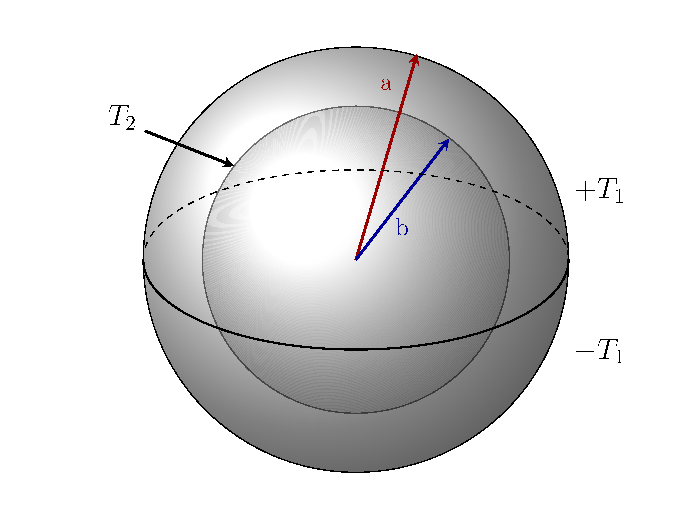
\includegraphics[scale=0.8]{Imagenes/esfera_8.eps}
    \caption{Los hemisferios de la esfera exterior de radio $a$ se encuentran a diferentes temperatura.}
    \label{fig:figura3}
\end{figure}
Calcula la temperatura:
\begin{enumerate}[label=\roman*)]
\item Dentro de la esfera interior,
\item En la región entre las dos esferas, y
\item Por fuera de la esfera exterior.
\end{enumerate}
\end{enumerate}

\end{document}